\documentclass[tikz,border=5pt]{standalone}
\usepackage{pgfplots}
\pgfplotsset{compat=1.18}
\usepgfplotslibrary{fillbetween}
\usetikzlibrary{arrows.meta,positioning,calc,decorations.pathreplacing,shapes.geometric}

\begin{document}
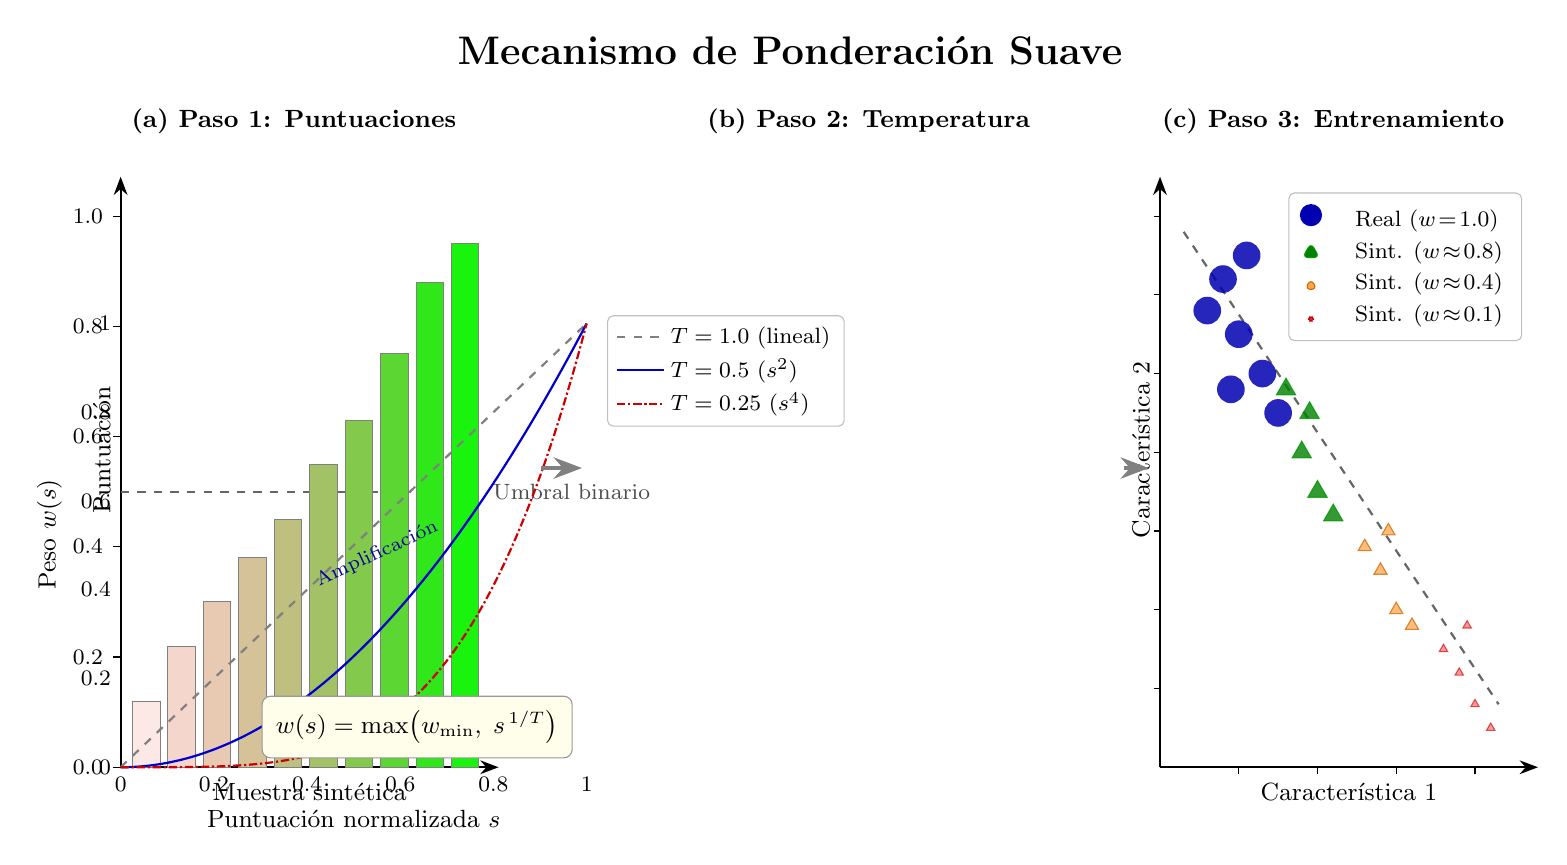
\begin{tikzpicture}[
    >=Stealth,
    font=\small,
    panel label/.style={font=\bfseries\small, align=center},
]

% ============================================================
% Global title
% ============================================================
\node[font=\Large\bfseries, anchor=south] at (8.5,8.8) {Mecanismo de Ponderaci\'{o}n Suave};

% ============================================================
% Panel (a): Paso 1 - Puntuaciones
% ============================================================
\begin{scope}[shift={(0,0)}]

  % Panel label
  \node[panel label] at (2.2,8.2) {(a) Paso 1: Puntuaciones};

  % Axes
  \draw[->, thick] (0,0) -- (0,7.5) node[midway, rotate=90, above=8pt] {Puntuaci\'{o}n};
  \draw[->, thick] (0,0) -- (4.8,0) node[below=2pt, pos=0.5] {Muestra sint\'{e}tica};

  % Y-axis ticks
  \foreach \y/\lab in {0/0.0, 1.4/0.2, 2.8/0.4, 4.2/0.6, 5.6/0.8, 7.0/1.0} {
    \draw (0,\y) -- (-0.1,\y) node[left, font=\footnotesize] {\lab};
  }

  % Threshold line
  \draw[dashed, thick, black!60] (0,3.5) -- (4.6,3.5)
    node[right, font=\footnotesize, text=black!70] {Umbral binario};

  % Bar data: 10 sorted scores
  % Scores: 0.12, 0.22, 0.30, 0.38, 0.45, 0.55, 0.63, 0.75, 0.88, 0.95
  \pgfmathsetmacro{\bw}{0.35}
  \foreach \i/\score/\r/\g in {
    1/0.12/90/10,
    2/0.22/80/20,
    3/0.30/70/30,
    4/0.38/60/40,
    5/0.45/50/50,
    6/0.55/40/60,
    7/0.63/30/70,
    8/0.75/20/80,
    9/0.88/10/90,
    10/0.95/5/95%
  } {
    \pgfmathsetmacro{\bh}{\score*7.0}
    \pgfmathsetmacro{\xpos}{0.15 + (\i-1)*0.45 + \bw/2}
    \fill[fill=red!\r!green!\g, draw=black!50, line width=0.3pt]
      (\xpos - \bw/2, 0) rectangle (\xpos + \bw/2, \bh);
  }

\end{scope}

% ============================================================
% Panel (b): Paso 2 - Temperatura (center, largest)
% ============================================================
\begin{scope}[shift={(6,0)}]

  % Panel label
  \node[panel label] at (3.5,8.2) {(b) Paso 2: Temperatura};

  \begin{axis}[
    at={(0,0)},
    anchor=south west,
    width=7.5cm,
    height=7.5cm,
    xmin=0, xmax=1,
    ymin=0, ymax=1.05,
    xlabel={Puntuaci\'{o}n normalizada $s$},
    ylabel={Peso $w(s)$},
    xlabel style={font=\small},
    ylabel style={font=\small},
    tick label style={font=\footnotesize},
    grid=both,
    grid style={gray!20},
    minor grid style={gray!10},
    legend style={
      at={(0.03,0.97)},
      anchor=north west,
      font=\footnotesize,
      draw=gray!50,
      fill=white,
      fill opacity=0.9,
      text opacity=1,
      rounded corners=2pt,
      cells={anchor=west},
    },
    axis on top,
    clip=false,
  ]

    % Fill between T=1.0 (linear) and T=0.5 (s^2) to show amplification
    \addplot[name path=linear, domain=0:1, samples=100, thick, dashed, gray]
      {x};
    \addlegendentry{$T=1.0$ (lineal)}

    \addplot[name path=Thalf, domain=0:1, samples=100, thick, blue!80!black, solid]
      {x^2};
    \addlegendentry{$T=0.5$ ($s^{2}$)}

    \addplot[name path=Tquarter, domain=0:1, samples=100, thick, red!80!black, densely dashdotted]
      {x^4};
    \addlegendentry{$T=0.25$ ($s^{4}$)}

    % Fill between linear and T=0.5
    \addplot[fill=blue!10, draw=none, forget plot]
      fill between[of=linear and Thalf, soft clip={domain=0:1}];

    % Annotation for amplification region
    \node[font=\scriptsize, text=blue!60!black, align=center, rotate=25]
      at (axis cs:0.55,0.48) {Amplificaci\'{o}n};

    % Formula box
    \node[
      draw=black!40,
      fill=yellow!8,
      rounded corners=3pt,
      font=\small,
      inner sep=5pt,
      anchor=south east,
    ] at (axis cs:0.97,0.02) {$w(s) = \max\!\big(w_{\min},\; s^{\,1/T}\big)$};

  \end{axis}

\end{scope}

% ============================================================
% Panel (c): Paso 3 - Entrenamiento
% ============================================================
\begin{scope}[shift={(13.2,0)}]

  % Panel label
  \node[panel label] at (2.2,8.2) {(c) Paso 3: Entrenamiento};

  % Axes
  \draw[->, thick] (0,0) -- (0,7.5) node[midway, rotate=90, above=8pt] {Caracter\'{i}stica 2};
  \draw[->, thick] (0,0) -- (4.8,0) node[below=2pt, pos=0.5] {Caracter\'{i}stica 1};

  % Tick marks
  \foreach \x in {1,2,3,4} {
    \draw (\x,0) -- (\x,-0.08);
  }
  \foreach \y in {1,2,3,4,5,6,7} {
    \draw (0,\y) -- (-0.08,\y);
  }

  % Decision boundary (dashed)
  \draw[dashed, thick, black!60] (0.3,6.8) -- (4.3,0.8);

  % Real data points: large blue circles (w=1.0)
  \foreach \x/\y in {0.8/6.2, 1.0/5.5, 1.3/5.0, 0.6/5.8, 1.5/4.5, 1.1/6.5, 0.9/4.8} {
    \fill[blue!70!black, opacity=0.85] (\x,\y) circle (5pt);
  }

  % Synthetic high-quality: medium green triangles (w~0.8)
  \foreach \x/\y in {1.8/4.0, 2.0/3.5, 1.6/4.8, 2.2/3.2, 1.9/4.5} {
    \node[draw=green!60!black, fill=green!50!black, opacity=0.8,
      regular polygon, regular polygon sides=3, minimum size=8pt, inner sep=0pt]
      at (\x,\y) {};
  }

  % Synthetic medium-quality: small orange triangles (w~0.4)
  \foreach \x/\y in {2.8/2.5, 3.0/2.0, 2.6/2.8, 3.2/1.8, 2.9/3.0} {
    \node[draw=orange!80!black, fill=orange!70, opacity=0.75,
      regular polygon, regular polygon sides=3, minimum size=5.5pt, inner sep=0pt]
      at (\x,\y) {};
  }

  % Synthetic low-quality: tiny red triangles (w~0.1)
  \foreach \x/\y in {3.8/1.2, 4.0/0.8, 3.6/1.5, 4.2/0.5, 3.9/1.8} {
    \node[draw=red!80!black, fill=red!60, opacity=0.65,
      regular polygon, regular polygon sides=3, minimum size=3.5pt, inner sep=0pt]
      at (\x,\y) {};
  }

  % Legend
  \node[
    draw=gray!50,
    fill=white,
    fill opacity=0.92,
    text opacity=1,
    rounded corners=2pt,
    inner sep=4pt,
    font=\footnotesize,
    anchor=north east,
    align=left,
  ] (leg) at (4.6,7.3) {
    \begin{tabular}{@{}cl@{}}
      \tikz\fill[blue!70!black] (0,0) circle (4pt); & Real ($w\!=\!1.0$) \\[2pt]
      \tikz\node[draw=green!60!black, fill=green!50!black, regular polygon,
        regular polygon sides=3, minimum size=7pt, inner sep=0pt] {}; & Sint. ($w\!\approx\!0.8$) \\[2pt]
      \tikz\node[draw=orange!80!black, fill=orange!70, regular polygon,
        regular polygon sides=3, minimum size=5pt, inner sep=0pt] {}; & Sint. ($w\!\approx\!0.4$) \\[2pt]
      \tikz\node[draw=red!80!black, fill=red!60, regular polygon,
        regular polygon sides=3, minimum size=3pt, inner sep=0pt] {}; & Sint. ($w\!\approx\!0.1$) \\
    \end{tabular}
  };

\end{scope}

% ============================================================
% Connecting arrows between panels
% ============================================================

% Arrow from panel (a) to panel (b)
\draw[->, ultra thick, black!50, shorten >=4pt, shorten <=4pt]
  (5.2, 3.8) -- (6.0, 3.8)
  node[midway, above, font=\scriptsize, text=black!60] {};

% Arrow from panel (b) to panel (c)
\draw[->, ultra thick, black!50, shorten >=4pt, shorten <=4pt]
  (12.6, 3.8) -- (13.2, 3.8)
  node[midway, above, font=\scriptsize, text=black!60] {};

\end{tikzpicture}
\end{document}
